\documentclass[11pt]{article}

\usepackage{bytefield}
\usepackage{hyperref}
\usepackage{csquotes}
\usepackage{url}
\usepackage{array,tabularx}
\usepackage{todonotes}
\usepackage{float}
\usepackage{tikz}
\usepackage{comment}
\usepackage{pgf-umlsd}

\usetikzlibrary{arrows,positioning,automata,calc}

\hypersetup{
    colorlinks=true,
    linkcolor=blue,
    filecolor=magenta,
    urlcolor=cyan,
}

\setlength{\parindent}{4em}
\setlength{\parskip}{1em}

\urlstyle{same}

\newcommand{\nanoarq}{\texttt{nanoarq}}

\begin{document}

\title{\nanoarq{}}
\author{Charles Nicholson \texttt{<\href{mailto:charles.nicholson@gmail.com}{charles.nicholson@gmail.com}>}}
\date{}
\maketitle

\begin{abstract}
    This document introduces \nanoarq{}, a single-file C library that provides reliability over an unreliable communications channel. \nanoarq{} implements the \href{https://en.wikipedia.org/wiki/Selective_Repeat_ARQ}{Selective Repeat ARQ} \todo{Cite ARQ}  algorithm and provides basic functionality for establishing and gracefully destroying connections. \nanoarq{} is meant to be suitable for embedded systems, with a design focus on simplicity, flexibility, and ease of integration. The \nanoarq{} implementation is released into the public domain.
\end{abstract}

\section{Introduction}
Many communications channels in embedded systems, such as UART lines between multiple CPUs, or between a target and host system, provide an unreliable transport for transmitting and receiving data. Bits can be altered in flight on the wire, in isolation or in bursts. Crosstalk and signal degradation can occur when the routing of critical signals is too long, or the signals are transmitted over cables. Even bytes that are transmitted without errors can be lost due to infrequent servicing of the transport layer, overwritten in a hardware register by the arrival of the next byte. Finally, application backpressure can cause valid incoming bytes to be discarded, as the system runs out of space to store them. \par
All of these problems speak to the necessity of a reliability layer in software. Sliding window protocols are the ubiquitous solution, and are used as the foundation for more complex protocols like TCP. Fundamentally, sliding window protocols guarantee that the application layer will be presented with all data that was sent to it, in order, with integrity and without duplicates. \par
\nanoarq{} is an implementation of the \enquote{Selective Repeat ARQ} protocol, and uses an explicit ACK mechanism to retransmit lost or corrupted frames. Additionally, \nanoarq{} provides connectivity services; a standard 3-way handshake and FIN/ACK disconnect strategy can be optionally used to establish and statefully manage a connection.

\subsection{Goals}
\begin{description}
\item[Reliability] \hfill \\
    First and foremost, \nanoarq{} provides reliability to unreliable communications. As long as the physical link still exists between the two endpoints, \nanoarq{} ensures that data will be transmitted in-order, without corruption, and without duplication of data.
\item[Simplicity] \hfill \\
    \nanoarq{} does as little work as possible to achieve its functionality, intentionally eschewing complex and powerful behavior that is present in TCP. \nanoarq{} is not a general-purpose networking toolkit; it exists only to provide reliability over a predictable link with reasonable performance between two endpoints.
\item[Transparency] \hfill \\
    \nanoarq{} does not hide implementation details from the user, or enforce a notion of encapsulation. \nanoarq{} is not object-oriented; all internal data structures are accessible to users. In the case the provided API does not offer sufficient functionality, it should be as easy as possible to access, manipulate, and extend \nanoarq{}'s state.
\item[Ease of Integration] \hfill \\
    \todo{shorten here, break details out into motivation / implementation section}
    It can be difficult to integrate third-party C libraries into a user application. The C language does not have a unified build system, which can have a \enquote{Tower of Babel} effect on attempts to reuse code. While packages like \texttt{CMake} and \texttt{Ninja} are growing in popularity, assuming their presence puts a significant burden on a would-be user. Additionally, deploying libraries on Windows with Visual Studio has the extra complexity of having to provide support for the static (\texttt{/MT}) and dynamic (\texttt{/MD}) versions of the Microsoft C Runtime. While some C libraries prefer to provide support for as many build systems as possible, \nanoarq{} aims to be as easy to integrate by providing no build system, instead existing in a single header file. This approach is prevalent and proven in Sean Barrett's \texttt{stb\_*} libraries. \par
    A similar challenge exists at runtime. \nanoarq{} is intended to be used in embedded systems, which have no standard operating system. Some systems run on so-called \enquote{bare metal} with a static task scheduling algorithm, while others may use sophisticated pre-emptive RTOS's that provide concurrency primitives, conditional waits, and work queues. \nanoarq{} is designed to work in any environment, as long as the user can provide the amount of time that has elapsed since the last polling call was made. \par
    Finally, the \nanoarq{} implementation and tests are released into the public domain, which means there are no licesnses or fees for use.
\end{description}

\subsection{Non-goals}
\begin{description}
\item[Implementing a Large Standard] \hfill \\
    \nanoarq{} does not aim to be a full TCP, IP, PPP, or POSIX-compatible sockets implementation. \nanoarq{} has no concept of routing, endpoints, ports, addresses, sockets, or names. \nanoarq{} clients do not statefully listen for connections; if a connection request arrives, it is serviced.
\item[Security] \hfill \\
    \nanoarq{} strives to be resilient against malformed input, but provides no encryption or authentication services. If security is required, it is up to the user to ensure that all data transmitted via \nanoarq{} is properly secured.
\item[Dynamic Configuration] \hfill \\
    \nanoarq{} assumes that both endpoints are compatibly configured. \nanoarq{} provides no services for communicating connection options during connection establishment.
\item[Congestion Control] \hfill \\
    \nanoarq{} is oblivious to the concept of congestive collapse, and performs no dynamic throttling of data in response to data loss. \nanoarq{} relies on the application to address the problems of congestion and backpressure.
\item[Physical Link Management] \hfill \\
    \nanoarq{} does not assume control over any specific communications hardware or OS resources. The user is responsible for the actual low-level transmission of bytes into and out of \nanoarq{}. This allows \nanoarq{} to function on embedded systems without requiring intimate knowledge of a given communication peripheral block, as well as on larger systems like desktop computers, across multiple operating systems, etc.
\item[Error Correction] \hfill \\
    \nanoarq{} does not currently support any form of forward error correction (e.g. Reed-Solomon, Turbocodes, etc.). A FEC encoding and reconstruction phase would be an interesting future addition to support environments that have an extremely high retransmission cost.
\end{description}

\section{Protocol}
\nanoarq{} implements a stream-based protocol, meaning that the internal delimiting and segmenting of data is not exposed to the application layer. As with the POSIX sockets API, users simply call functions similar to \texttt{send()} and \texttt{recv()}. There is no parity guarantee between the transmitter's \texttt{send()} calls and receiver's \texttt{recv()} calls. \par
Internally, \nanoarq{} breaks up transmissions into fixed-size blocks so that they can be selectively acknowledged. The atomic unit of transmitted data is the \texttt{frame}. The portion of the frame that carries the user data is called the \texttt{segment}. A \texttt{message} is an aggregation of frames, and the unit of acknowledgement. It is the user's responsibility to configure \nanoarq{} to find a balance between message size and window size to maximize bandwidth and minimize unnecessary acknowledgement traffic. \par

\subsection{Frames}
Frames contain a header, a segment, and an optional checksum footer. The frame header carries enough information to uniquely identify which message it belongs to. It also carries the sender's receive window size for flow control purposes. The frame layout is visible in figure~\ref{fig:frame-layout}. Frames are encoded using the COBS algorithm to ensure that frame delimiting is unambiguous, but does impose a maximum frame size of 254 bytes. Frame headers and footers consume a maximum of 16 bytes, so the maximum payload size per segment is 238 bytes. Accordingly, \nanoarq{} introduces a 6.7\% overhead on transmission size. \\ \par

\begin{figure}[H]
\begin{bytefield}[bitwidth=1.1em,bitheight=2em]{32}
	\bitheader{0-31} \\
    \bitbox{8}{Version} & \bitbox{8}{Payload Size} & \bitbox{5}{Reserved} & \bitbox{1}{\tiny R\\S\\T} & \bitbox{1}{\tiny A\\C\\K} & \bitbox{1}{\tiny F\\I\\N} & \bitbox{8}{Window Size} \\
    \bitbox{12}{Sequence Number} & \bitbox{8}{Segment Count} & \bitbox{12}{Segment ID} \\
    \bitbox{12}{ACK Number} & \bitbox{8}{Reserved} & \bitbox{12}{ACK Segment Mask} \\
    \wordbox[lrt]{1}{Payload Octets} \\
    \skippedwords \\
    \wordbox[lrb]{1}{} \\
    \bitbox{32}{Checksum (optional)}
\end{bytefield}
\caption{\nanoarq{} frame layout}
\label{fig:frame-layout}
\end{figure}

A description of each field follows.
\begin{description}
\item[Version] \hfill \\
\item[Payload Size] \hfill \\
\item[Flags] \hfill \\
\item[Window Size] \hfill \\
\item[Sequence Number] \hfill \\
\item[Segment Count] \hfill \\
\item[Segment ID] \hfill \\
\item[ACK Number] \hfill \\
\item[ACK Segment Mask] \hfill \\
\item[Payload Octets] \hfill \\
\item[Checksum] \hfill \\
\end{description}

\subsection{Messages}
\subsection{Connection State Machine}
\begin{figure}
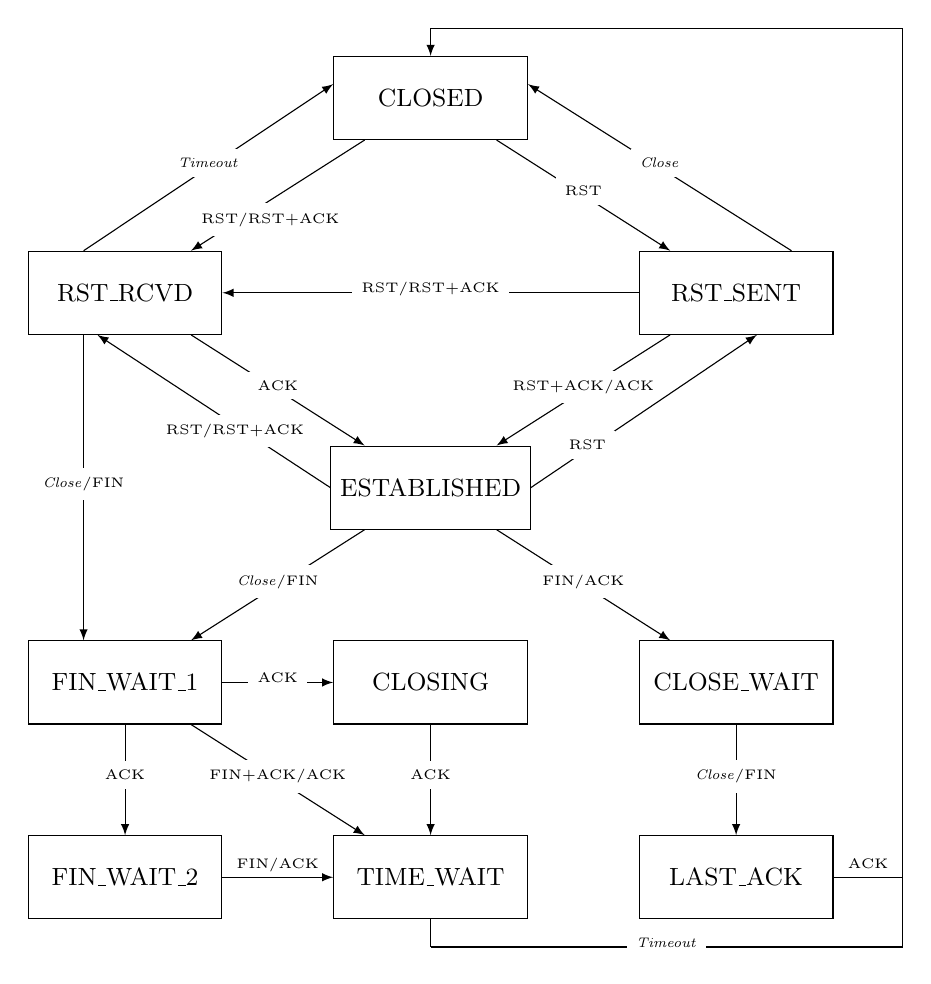
\begin{tikzpicture}[auto]

\tikzset{every node/.style = {font=\tiny,fill=white,above,anchor=base}}
\tikzset{every edge/.append style = {>=latex}}
\tikzstyle{state} = [rectangle, minimum height=3em, minimum width=7em, node distance=4em, font=\small]

\node[state, draw] (closed)                      {CLOSED};
\node[state]       (anchor)  [below= of closed]  {};
\node[state, draw] (rst_s)   [right= of anchor]  {RST\_SENT};
\node[state, draw] (rst_r)   [left= of anchor]   {RST\_RCVD};
\node[state, draw] (est)     [below= of anchor]  {ESTABLISHED};
\node[state, draw] (closing) [below= of est]     {CLOSING};
\node[state, draw] (fin_w1)  [left= of closing]  {FIN\_WAIT\_1};
\node[state, draw] (fin_w2)  [below= of fin_w1]  {FIN\_WAIT\_2};
\node[state, draw] (close_w) [right= of closing] {CLOSE\_WAIT};
\node[state, draw] (last_a)  [below= of close_w] {LAST\_ACK};
\node[state, draw] (time_w)  [below= of closing] {TIME\_WAIT};

\draw (closed)                      edge[->] node[pos=0.75,xshift=1.3em] {RST/RST+ACK}      (rst_r);
\draw (closed)                      edge[->] node                        {RST}              (rst_s);
\draw ($(rst_r.south) - (1.5em,0)$) edge[->] node                        {\emph{Close}/FIN} ($(fin_w1.north) - (1.5em,0)$);
\draw (rst_r)                       edge[->] node                        {ACK}              (est);
\draw ($(rst_r.north) - (1.5em,0)$) edge[->] node                        {\emph{Timeout}}   ($(closed.west) + (0,0.5em)$);
\draw (rst_s)                       edge[->] node                        {RST+ACK/ACK}      (est);
\draw (rst_s.west)                  edge[->] node                        {RST/RST+ACK}      (rst_r.east);
\draw ($(rst_s.north) + (2em,0)$)   edge[->] node                        {\emph{Close}}     ($(closed.east) + (0,0.5em)$);
\draw (est)                         edge[->] node                        {\emph{Close}/FIN} (fin_w1);
\draw (est)                         edge[->] node                        {FIN/ACK}          (close_w);
\draw (est.east)                    edge[->] node[pos=0.25]              {RST}              ($(rst_s.south) + (0.75em,0)$);
\draw (est.west)                    edge[->] node[pos=0.35,xshift=-.5em] {RST/RST+ACK}      ($(rst_r.south) - (1em,0)$);
\draw (fin_w1.south)                edge[->] node                        {ACK}              (fin_w2.north);
\draw (fin_w1.east)                 edge[->] node                        {ACK}              (closing);
\draw (fin_w1)                      edge[->] node                        {FIN+ACK/ACK}      (time_w);
\draw (fin_w2)                      edge[->] node[yshift=0.3em,fill=none]{FIN/ACK}          (time_w);
\draw (closing)                     edge[->] node                        {ACK}              (time_w);
\draw (close_w)                     edge[->] node                        {\emph{Close}/FIN} (last_a);

\coordinate (south_east) at ($(last_a.east |- last_a.south) + (2.5em,-1em)$);
\coordinate (north_east) at ($(closed.north -| south_east) + (0,1em)$);
\coordinate (above_closed) at ($(closed.north) + (0,1em)$);
\coordinate (last_a_closed_1) at ($(last_a.east) + (2.5em,0)$);
\coordinate (time_w_closed_1) at ($(time_w.south) + (0,-1em)$);

\draw (last_a.east)                 edge     node[yshift=0.3em,fill=none]{ACK}              (last_a_closed_1);
\draw (south_east)                  edge                                                    (north_east);
\draw (north_east)                  edge                                                    (above_closed);
\draw (above_closed)                edge[->]                                                (closed);
\draw (time_w.south)                edge                                                    (time_w_closed_1);
\draw (time_w_closed_1)             edge     node                        {\emph{Timeout}}   (south_east);

\end{tikzpicture}
\caption{\nanoarq{} state machine}
\label{fig:state-machine}
\end{figure}
\nanoarq{} optionally provides stateful connection services for establishing, maintaining, and closing a connection to the peer endpoint. The state machine, detailed in figure~\ref{fig:state-machine}, is similar to TCP but differs slightly. \nanoarq{} has no concept of a client or a server, so the \texttt{LISTEN} state present in TCP does not exist. There is also no distinction between connecting and resetting, so the difference between \texttt{RST} and \texttt{SYN} is uninteresting.

\subsection{Flow Control}

\section{Physical Organization}
\end{document}
